\section{What a Force Close Costs}
\label{sec:cost}

\begin{table*}[t]
\centering
\caption{What a public force close costs, against a cooperative close, 2019--2026 (medians, sat unless stated).}
\label{tab:costs}
\footnotesize
\begin{tabular}{lrrrrrrrrrr}
\toprule
Year & Force closes & Commit. & Total & p90 & Coop. & Ratio & vB & Coop.\ vB & >1\% cap. & Days \\
\midrule
2019 & 30{,}001 & 4{,}900 & 7{,}460 & 24{,}802 & 3{,}485 & 2.1 & 270 & 138 & 54.9 & 1.0 \\
2020 & 17{,}813 & 9{,}051 & 14{,}318 & 36{,}545 & 3{,}994 & 3.6 & 271 & 168 & 63.1 & 1.0 \\
2021 & 27{,}393 & 2{,}583 & 3{,}984 & 31{,}397 & 697 & 5.7 & 302 & 168 & 41.0 & 1.0 \\
2022 & 57{,}896 & 2{,}021 & 3{,}342 & 7{,}920 & 551 & 6.1 & 521 & 169 & 16.1 & 1.7 \\
2023 & 49{,}998 & 2{,}872 & 7{,}346 & 45{,}588 & 2{,}005 & 3.7 & 595 & 192 & 32.1 & 2.1 \\
2024 & 28{,}888 & 3{,}012 & 6{,}332 & 36{,}635 & 2{,}124 & 3.0 & 581 & 192 & 29.6 & 2.0 \\
2025 & 21{,}518 & 730 & 1{,}292 & 3{,}912 & 262 & 4.9 & 598 & 192 & 11.7 & 1.7 \\
2026\textsuperscript{a} & 14{,}435 & 597 & 925 & 2{,}363 & 197 & 4.7 & 585 & 192 & 7.5 & 2.5 \\
\bottomrule
\end{tabular}
\par\smallskip\parbox{\linewidth}{\scriptsize \textsuperscript{a}Closes to 4 October 2026, so that outputs had four weeks to be spent. Total: every fee the force close requires (commitment, fee bump, HTLC resolution, sweeps, anchor cleanup); batched spends split per input. Ratio: median total over the median cooperative close fee. vB: block space, the same way. $>$1\% cap.: share of force closes whose fees exceed 1\% of channel capacity. Days: median wait before the broadcaster's own balance can be swept.}
\end{table*}


\begin{figure*}[t]
\centering
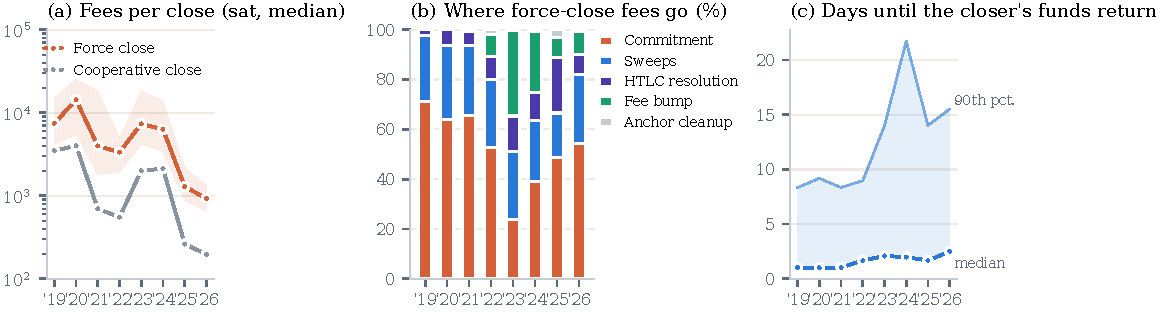
\includegraphics[width=\textwidth]{figures/fig3_costs.pdf}
\caption{The cost of a public force close. (a) Median fees per close, force and cooperative (log scale; band:
interquartile range of force closes). (b) Where force-close fees go: the commitment, sweeps of the broadcaster's
balance and of anchor channels' \texttt{to\_remote}, HTLC resolution, fee bumps (owner CPFP children in the
commitment's block) and later anchor cleanup. (c) Days until the broadcaster's own balance can be swept: median and
90th percentile.}
\label{fig:costs}
\end{figure*}

\subsection{Fees, time and block space}

\paragraph{Cheap in fees, a multiple of a cooperative close}
In fees alone a force close is cheap: the median public force close cost \CostMedTwentySix~sat in 2026
(Table~\ref{tab:costs}). The median was highest in 2020, at \CostMedTwenty~sat, against \CostMedTwentyThree~sat in
2023. Against a cooperative close of the same year it is dear: \CostRatioMin--\CostRatioMax{} times the median
cooperative close in every year. The fee market sets the level, not the ratio. Force closes paid
\CostTotalBtcAll~BTC in fees over the whole period, \CostTotalBtcTwentyThree~BTC of it in 2023, more than in any other
year.

\paragraph{When fees are high, the money goes to bumps and HTLCs}
In 2023, fee bumps took \BumpShareTwentyThree\% of all force-close fees and HTLC resolution \HtlcShareTwentyThree\%
(Fig.~\ref{fig:costs}b). That year \AnchorBumpedPctTwentyThree\% of anchor force closes were bumped by a child in the
commitment's block, and \BumpPctHtlcTwentyThree\% of those with pending HTLCs. In the low-fee years the commitment
and the sweeps make up most of the cost.

\paragraph{Anchors doubled the block space}
An anchor force close uses about twice the block space of a pre-anchor one (median \AnchorVbMed{} against
\LegacyVbMed~vB): two extra outputs, a \texttt{to\_remote} output that needs a sweep of its own, and the anchors'
spends. Since 2022 a force close has taken \VbRatioMin--\VbRatioMax{} times the block space of a cooperative close.
Block space does not depend on the fee regime, which makes it the currency in which formats compare most directly
(\S\ref{sec:zerofee}).

\paragraph{The closer waits days}
The broadcaster's own balance returns a median \ToLocalMedDays{} days after the close, and in the slowest tenth of
closes up to \ToLocalPNinetyMax{} days (Fig.~\ref{fig:costs}c). The wait is the \texttt{to\_self\_delay} the peer chose
at opening: \DelayOneDayPct\% of values are 144 blocks (one day) and \DelayTwoWeeksPct\% about two weeks. Over the
period, closers' balances were locked for \BtcDaysLockedAll{} BTC-days.

\paragraph{The wait outweighs the fees only when fees are low}
The break-even rate was \BreakEvenRateTwentyFive\% in 2025 and \BreakEvenRateTwentySix\% in 2026, so in the low-fee
years even a modest return on the locked funds made the wait the larger cost. Before 2025 it was
\BreakEvenRateEarlyMin--\BreakEvenRateEarlyMax\% a year. Over the whole period the wait cost more than the fees only
for funds earning more than \BreakEvenRateAll\% a year.

\paragraph{Relative to capacity, the cost fell}
In 2021, \OverOnePctCapTwentyOne\% of public force closes paid more than 1\% of the channel's capacity in fees; in
2026, \OverOnePctCapTwentySix\%.

\subsection{Penalties and a breach wave}
\label{sec:breach}

\paragraph{Penalties are rare}
Over the period, \PenaltyTxsAll{} penalty transactions took \PenaltyBtcAll~BTC from parties that broadcast a revoked
commitment, in public or private channels. Until September~2026 a typical month had \PenaltyMonthlyMed{} and none
had more than \PenaltyMonthlyMaxBefore{} (\PenaltyMonthlyMaxBeforeMonth). Only punished breaches are visible: a breach
that went unpunished looks like an ordinary force close.

\paragraph{A one-week breach wave}
Between \PenaltyWaveFirst{} and \PenaltyWaveLast, revoked commitments of \BreachWavePenalised{} private anchor
channels were broadcast, and every one was penalized within \PenaltyWaveMaxBlocks{} blocks. \BreachWaveChannels{} of
them (\BreachWaveBtc~BTC) were splices of channels opened a median of \BreachOpenToSpliceMed{} blocks earlier by one
funder, which also collected the penalties. The counterparty force-closed about \BreachSpliceToCloseMed{} blocks after
each splice; \BreachLookAlikesWeek{} more such closes that week used the current state. The remaining channel is an
unrelated breach of an older channel. The transactions on both sides follow Core Lightning's construction rules, and
the wave matches a bug that Core Lightning fixed in version 26.06.8, released on 19~September~2026~\cite{cln26068}. In
affected versions, a unilateral close after a splice had locked broadcast the commitment from the moment of the lock,
which is revoked as soon as the channel is updated again. Core Lightning locks a splice at three confirmations, which
is when the closes came. The bug explains why the old states were always post-splice states and why some closes used
the current state. The chain does not show what made each counterparty close at the lock, or whether the funder
caused it. This one week holds most of 2026's \PenaltyTxsTwentySix{} penalties and is the only
event of its kind in our data, which go back to 2018.

\subsection{Exposure: HTLC deadlines}
\label{sec:htlc}

\begin{figure*}[t]
\centering
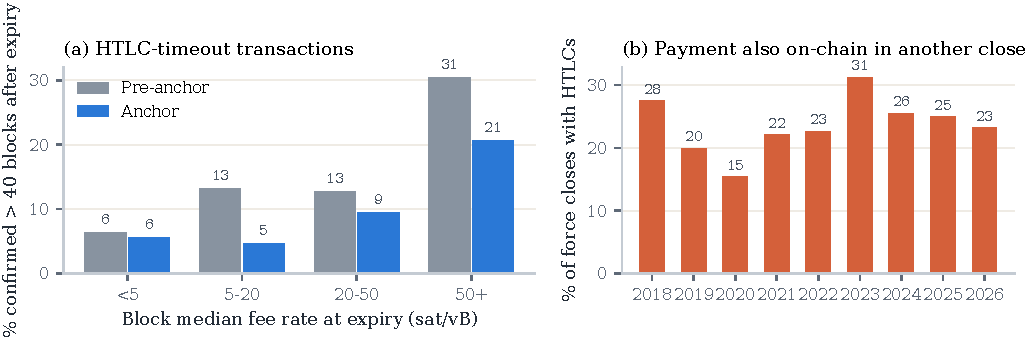
\includegraphics[width=0.85\textwidth]{figures/fig7_htlc_deadlines.pdf}
\caption{HTLCs resolved on-chain. (a) Share of HTLC-timeout transactions confirmed more than \HtlcMarginTight{}
blocks after the HTLC's expiry, by the median fee rate of the block at expiry, for pre-anchor and anchor channels
whose commitment had confirmed by the expiry. (b) Share of force closes with an HTLC resolved on-chain whose payment
also appears in another force close, by year.}
\label{fig:htlc}
\end{figure*}

\paragraph{Most HTLC timeouts are prompt; the late tail grows with fees}
Of \HtlcTimeoutTxs{} HTLC-timeout transactions, the median confirmed \HtlcTimeoutMedMin--\HtlcTimeoutMedMax{} blocks
after its expiry in every year. The tail is what matters for a forwarding node. More than \HtlcMarginTight{} blocks
late were \HtlcLateEarlyMin--\HtlcLateEarlyMax\% of timeouts in each year from 2019 to 2022, then
\HtlcLateTwentyThree\% in 2023, the high-fee year, and \HtlcLateTwentyFour\% in 2024. In \HtlcCommitBeforeExpiryPct\%
of cases the commitment had confirmed before the expiry, so the delay was the HTLC transaction's own.

\paragraph{Anchors keep HTLC timeouts closer to the deadline when fees are high}
When the block median fee rate at expiry was 50~sat/vB or more, \HtlcLateSpikeLegacy\% of pre-anchor HTLC timeouts
confirmed more than \HtlcMarginTight{} blocks late, against \HtlcLateSpikeAnchor\% of anchor ones
(Fig.~\ref{fig:htlc}a). At 5--20~sat/vB the gap was \HtlcLateMidLegacy\% against \HtlcLateMidAnchor\%; below
5~sat/vB the two formats were alike. A pre-anchor HTLC transaction carries the fee fixed at signing, while an anchor
channel's can add inputs to pay a fee chosen at broadcast. This is the effect the anchor design was built for, and
unlike the commitment-level test of \S\ref{sec:fees} it shows up in the data.
The exception is 2024, when anchor channels' timeouts were late more often than pre-anchor ones
(\HtlcLateTwentyFourAnchor\% against \HtlcLateTwentyFourLegacy\%).

\paragraph{Successes mostly come early}
HTLC-success transactions confirmed a median \HtlcSuccessMarginMin--\HtlcSuccessMarginMax{} blocks before expiry in
every year. In most years only \HtlcSuccessLateMinOther--\HtlcSuccessLateMaxOther\% came at or after the expiry, when
the peer can already take the HTLC back. Three years had more: \HtlcSuccessLateTwentyFour\% in 2024,
\HtlcSuccessLateNineteen\% in 2019 and \HtlcSuccessLateTwentyThree\% in 2023.

\paragraph{One payment can take several channels on-chain}
The payment hash links one payment's HTLCs across closes (\S\ref{sec:htlc-method}). Of the force closes with an HTLC resolved on-chain, \CascadePct\% share a payment with another force close
(Fig.~\ref{fig:htlc}b): \CascadePayments{} payments, up to \CascadeMaxCloses{} closes for one payment, with a median
of \CascadeSpanMed{} blocks between the first and the last. \CascadeAllTimeoutPct\% of them were timed out on every
channel: a stuck payment, or the parts of one multi-part payment, taking several channels down along its route.

\paragraph{Split resolutions are rare losses}
From \SplitResFromYear, in \SplitResPayments{} payments a forwarding node's two HTLCs were resolved in opposite ways:
with the preimage on one channel and by timeout on the other, so one party lost the HTLC amount (\SplitResBtc~BTC in
all). In \SplitResForwarderPayments{} of them (\SplitResForwarderBtc~BTC) the upstream HTLC timed out while the
downstream one was paid, so the node between them paid out and was not paid; in \SplitResPreimageFirstPct\% of those
the preimage was already on-chain a median \SplitResGapMed{} blocks before the upstream timeout confirmed. The losses
do not cluster in the 2023 fee spike, which points at nodes that were offline or failed to act rather than at fee
competition. These counts leave out \SplitResStagedPairs{} pairs from 2026 (\SplitResStagedBtc~BTC) whose channels
used a \SplitResStagedToSelfDelay-block \texttt{to\_self\_delay}: a replacement-cycling test, described next, not
organic losses.

\paragraph{No loss has the order replacement cycling leaves}
In a replacement-cycling attack the downstream peer keeps replacing the forwarder's HTLC-timeout transaction in the
mempool, and lets its own preimage claim confirm only after the upstream HTLC has timed
out~\cite{riard2023replacement}. A successful attack therefore puts the preimage on-chain after the upstream timeout.
No forwarder loss from \SplitResFromYear{} has that order. The staged pairs do, and they are such an attack, run as a
test: one operator ran the upstream, forwarding and downstream nodes and cycled its own forwarder's HTLC-timeout
transactions on mainnet. Shared funding and direct transfers link the three nodes' wallets, and the transactions that
evicted the forwarder's timeouts carry a fingerprint we find nowhere else on the chain in that period. In each staged
pair the preimage confirmed no earlier than the upstream timeout, a median of \SplitResStagedPreimageAfterMed{} blocks
after. The test sees only
payments whose two HTLCs were both resolved on-chain, so it bounds attacks that succeeded that way, not attempts.

\subsection{The whole life of a channel}
\label{sec:lifecycle}

\begin{table*}[t]
\centering
\caption{What a public channel's life costs on-chain: funding share, close and required spends, by year of close (medians, sat unless stated).}
\label{tab:lifecycle}
\footnotesize
\begin{tabular}{lrrrrrrrrrrr}
\toprule
Closed & Channels & Force \% & Open & Coop. & Force & All & Range & p90 & \% cap. & Opens \% & BTC \\
\midrule
2019 & 60{,}405 & 49.7 & 2{,}429 & 8{,}322 & 11{,}021 & 9{,}581 & 7{,}842--9{,}581 & 28{,}253 & 1.29 & 36.3 & 8.00 \\
2020 & 46{,}598 & 38.2 & 2{,}362 & 9{,}061 & 19{,}174 & 12{,}750 & 10{,}708--12{,}750 & 38{,}299 & 1.51 & 36.6 & 8.55 \\
2021 & 91{,}441 & 30.0 & 925 & 2{,}127 & 8{,}329 & 3{,}368 & 2{,}701--3{,}368 & 30{,}606 & 0.39 & 47.0 & 10.11 \\
2022 & 150{,}542 & 38.5 & 361 & 1{,}162 & 4{,}249 & 2{,}153 & 1{,}790--2{,}153 & 7{,}859 & 0.10 & 44.9 & 6.04 \\
2023 & 112{,}481 & 44.5 & 1{,}069 & 3{,}864 & 10{,}119 & 6{,}106 & 5{,}090--6{,}106 & 33{,}969 & 0.22 & 30.0 & 20.51 \\
2024 & 79{,}763 & 36.2 & 2{,}290 & 5{,}544 & 10{,}710 & 7{,}032 & 5{,}437--7{,}032 & 31{,}803 & 0.18 & 44.3 & 14.07 \\
2025 & 79{,}656 & 27.0 & 477 & 907 & 2{,}374 & 1{,}261 & 937--1{,}261 & 5{,}331 & 0.03 & 62.0 & 2.40 \\
2026\textsuperscript{a} & 71{,}639 & 20.1 & 309 & 626 & 1{,}450 & 785 & 569--785 & 2{,}927 & 0.01 & 64.6 & 1.24 \\
\midrule
All & 692{,}525 & 35.8 & 723 & 1{,}970 & 6{,}645 & 3{,}435 & 2{,}804--3{,}435 & 23{,}171 & 0.15 & 39.7 & 70.92 \\
\bottomrule
\end{tabular}
\par\smallskip\parbox{\linewidth}{\scriptsize \textsuperscript{a}Closes to 4 October 2026 (four weeks for outputs to be spent). Open: the channel's share of its funding transaction's fee, split equally over the channel outputs of the transaction; other outputs are the funder's change and pay nothing. Range: the median lifecycle if every output, change included, pays for its own size, and with the equal split. Coop., Force: lifecycles ending in a cooperative or a force close; force closes as in Table~II. \% cap.: median lifecycle fees over capacity. Opens \%: opens' share of all lifecycle fees. BTC: all lifecycle fees. Closes from 2019: our list of public channels holds few of the channels that closed in 2018.}
\end{table*}


\begin{figure*}[t]
\centering
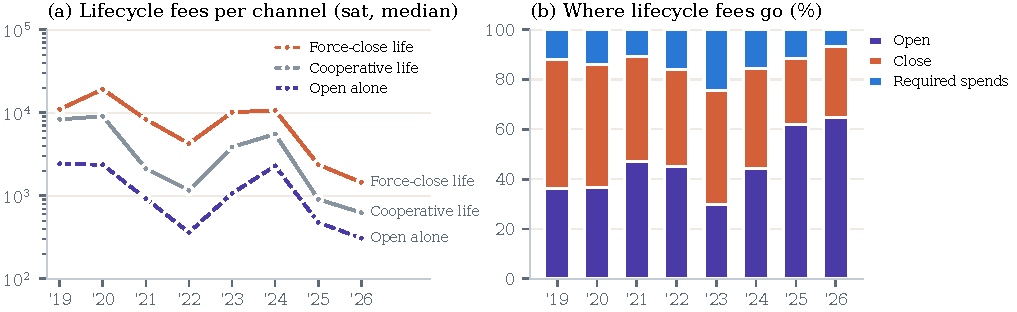
\includegraphics[width=0.85\textwidth]{figures/fig8_lifecycle.pdf}
\caption{A public channel's on-chain fees from funding to its last required spend. (a) Median by year of close, for
lives ending in a force close or a cooperative close, and the channel's share of its funding transaction alone (log
scale). (b) Where lifecycle fees go: the open, the close and the spends a force close requires.}
\label{fig:lifecycle}
\end{figure*}

\paragraph{A channel's life costs a few thousand satoshis}
Funding, closing and the spends a force close requires cost a public channel a median of \LcMed~sat
(Table~\ref{tab:lifecycle}): \LcOpenMed{} for its share of the funding transaction and \LcCloseMed{} for the close.
The median life cost \LcCapPct\% of the channel's capacity. The fee regime dominates. Channels closed in 2019--20 paid
the most, a median \LcMedEarlyRegime~sat; those closed in 2023--24 paid \LcMedHighRegime, and those closed in 2025--26
\LcMedLowRegime.

\paragraph{The open is a large part of the bill}
Opens paid \LcOpensPct\% of all lifecycle fees (\LcOpenBtc{} of \LcTotalBtc~BTC), and \LcOpensPctLowRegime\% for the
channels closed in 2025--26, which closed cheaply but had often opened in dearer blocks (Fig.~\ref{fig:lifecycle}b).

\paragraph{Counting the open narrows the gap between endings}
A life that ended cooperatively cost a median \LcCoopMed~sat, one that ended in a force close \LcForceMed{}, a ratio of
\LcForceCoopRatio{} (\LcForceCoopRatioMin--\LcForceCoopRatioMax{} by year), against \CostRatioMin--\CostRatioMax{}
for the close alone, because both kinds of channel paid the same to open. If change outputs also paid their share of
the funding fee, by value or by size, the median life would cost \LcRobustMinPct--\LcRobustMaxPct\% less; treating
funding transactions that also pay others as payment batches moves it by \LcRobustBatchPct\%. The lifecycles are
completed ones, so they favour short-lived channels (median life \LcLifeDaysMed{} days).
